\documentclass{ime-beamer}
\usepackage[portuges]{babel}
\usepackage[utf8]{inputenc}
\usepackage{graphicx}
\usepackage[portuguese]{algorithm2e}% Para escrever algorítimos
\usepackage{listings}			% Para usar \lstinputlisting e incluir código
%\usepackage{subcaption}			% Para usar \begin{subfigure} e colocar figuras (a) e (b) lado a lado
\usepackage{multicol}

\title[Uma Ferramenta para Futebol de Robôs]{Uma Ferramenta de Representação Comportamental Baseada em Otimização para Futebol de Robôs}
\author[Jan Segre\and Victor Bramigk]{%
  Jan Segre\\
  Victor Bramigk\\
  Paulo F. F. Rosa (Orientador)\\
  Bruno Eduardo Madeira (Coorientador)
}

% as imagens ficam nesse diretório
\graphicspath{{img/}}

\begin{document}
\frame{\maketitle}

\frame{%
  \frametitle{Roteiro}
  \tableofcontents
}

\section{Introdução}
% Robocup
% Objetivo
\frame{%
  \frametitle{Robocup}
  \begin{block}{}
    \begin{figure}
      \centering
      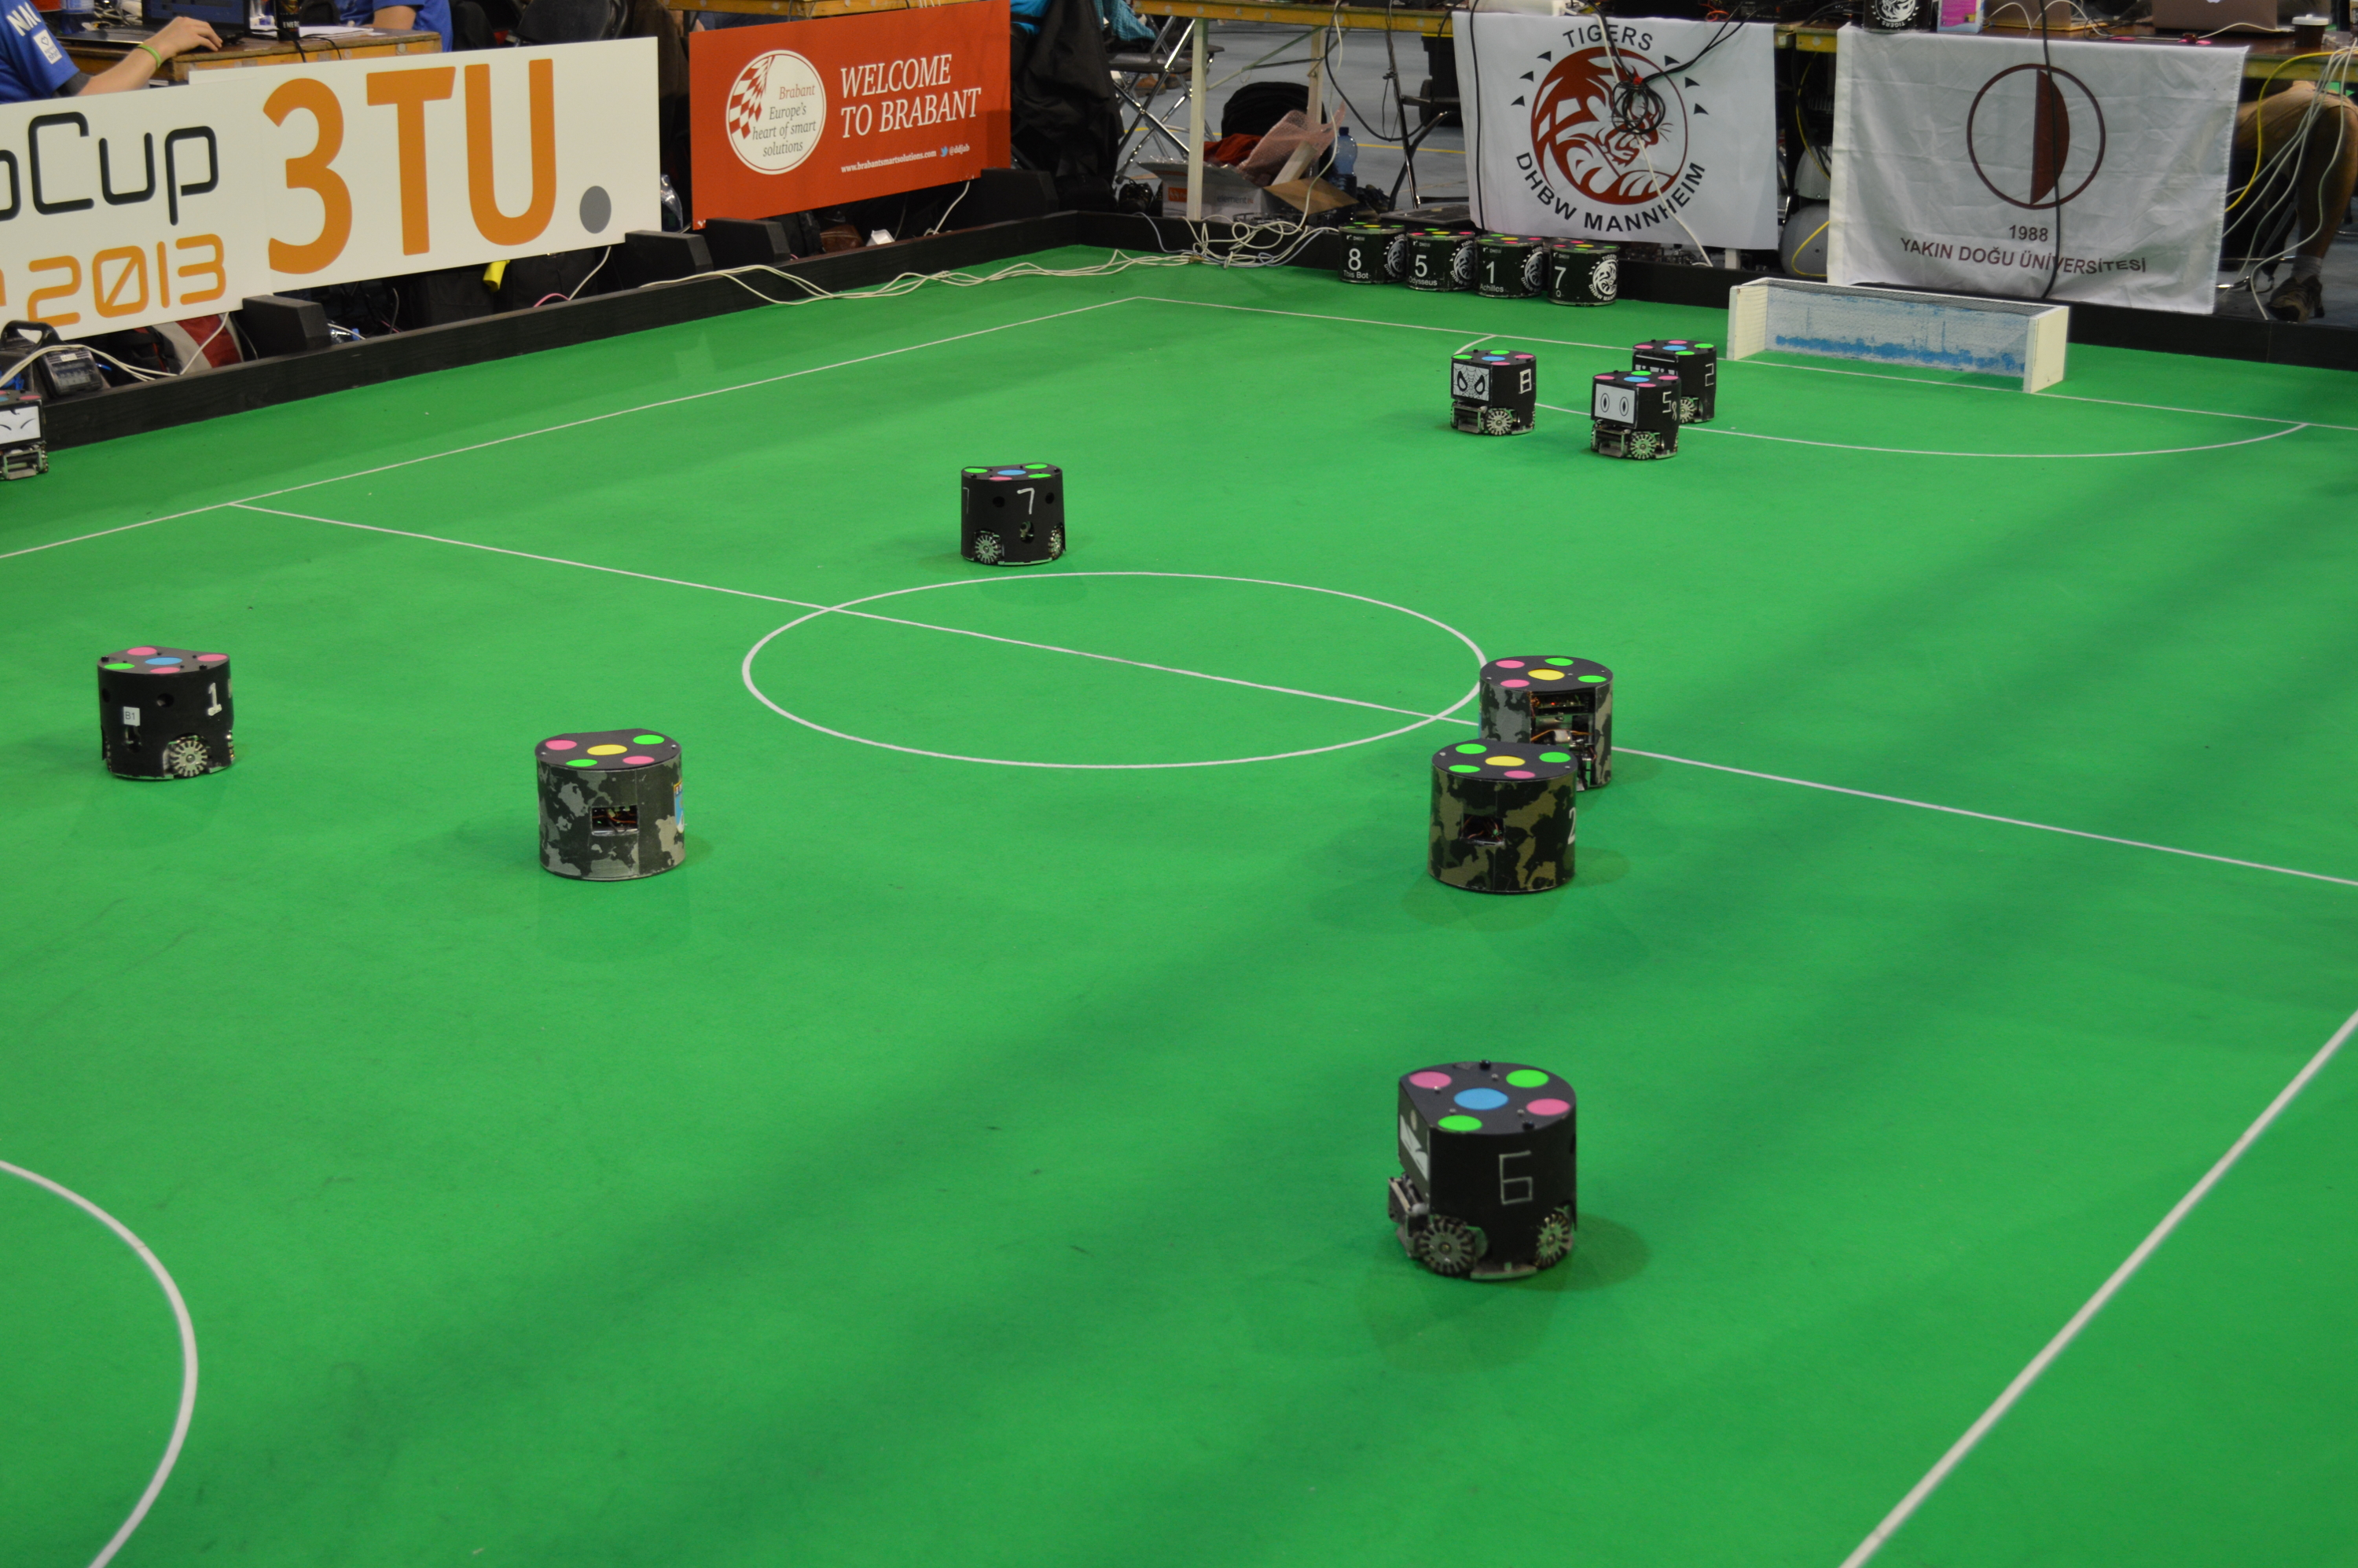
\includegraphics[width=0.7\linewidth]{robocup2013}
      \caption{Imagem da SSL \textit{RoboCup} 2013 em Eindhoven, na Holanda}\label{fig:robocup2013}
    \end{figure}
  \end{block}
}

\frame{%
  \frametitle{Objetivo}
  \begin{block}
    \centering
    \begin{itemize}
      \item Desenvolver uma ferramenta de representação
        comportamental baseado em otimização para futebol de robôs

      \item Criar um modelo discreto sequencial para o
        problema do futebol de robôs
    \end{itemize}
  \end{block}
}

\section{Modelagem}
% Modelagem
% tempo: X min
% - SSL
% - Definições
% |--> Posse de bola
% +--> Move Pass Kick
% - Discretização
% - Função Objetivo
% - Estratégia de Busca
\frame{%
  \frametitle{Modelagem}
  \begin{block}{}
    \centering
    \begin{itemize}
      \item SSL
      \item Definições
      \item Discretização
      \item Função Objetivo
      \item Estratégia de Busca
    \end{itemize}
  \end{block}
}

\subsection{SSL}
\frame{%
  \frametitle{SSL}
  \begin{figure}[thpb]
    \includegraphics[width= 0.8\linewidth]{img/cmra_campo}
    \caption{Disposição das câmeras no campo}
  \end{figure}
}
\frame{%
  \frametitle{SSL}
  \begin{figure}[thpb]
    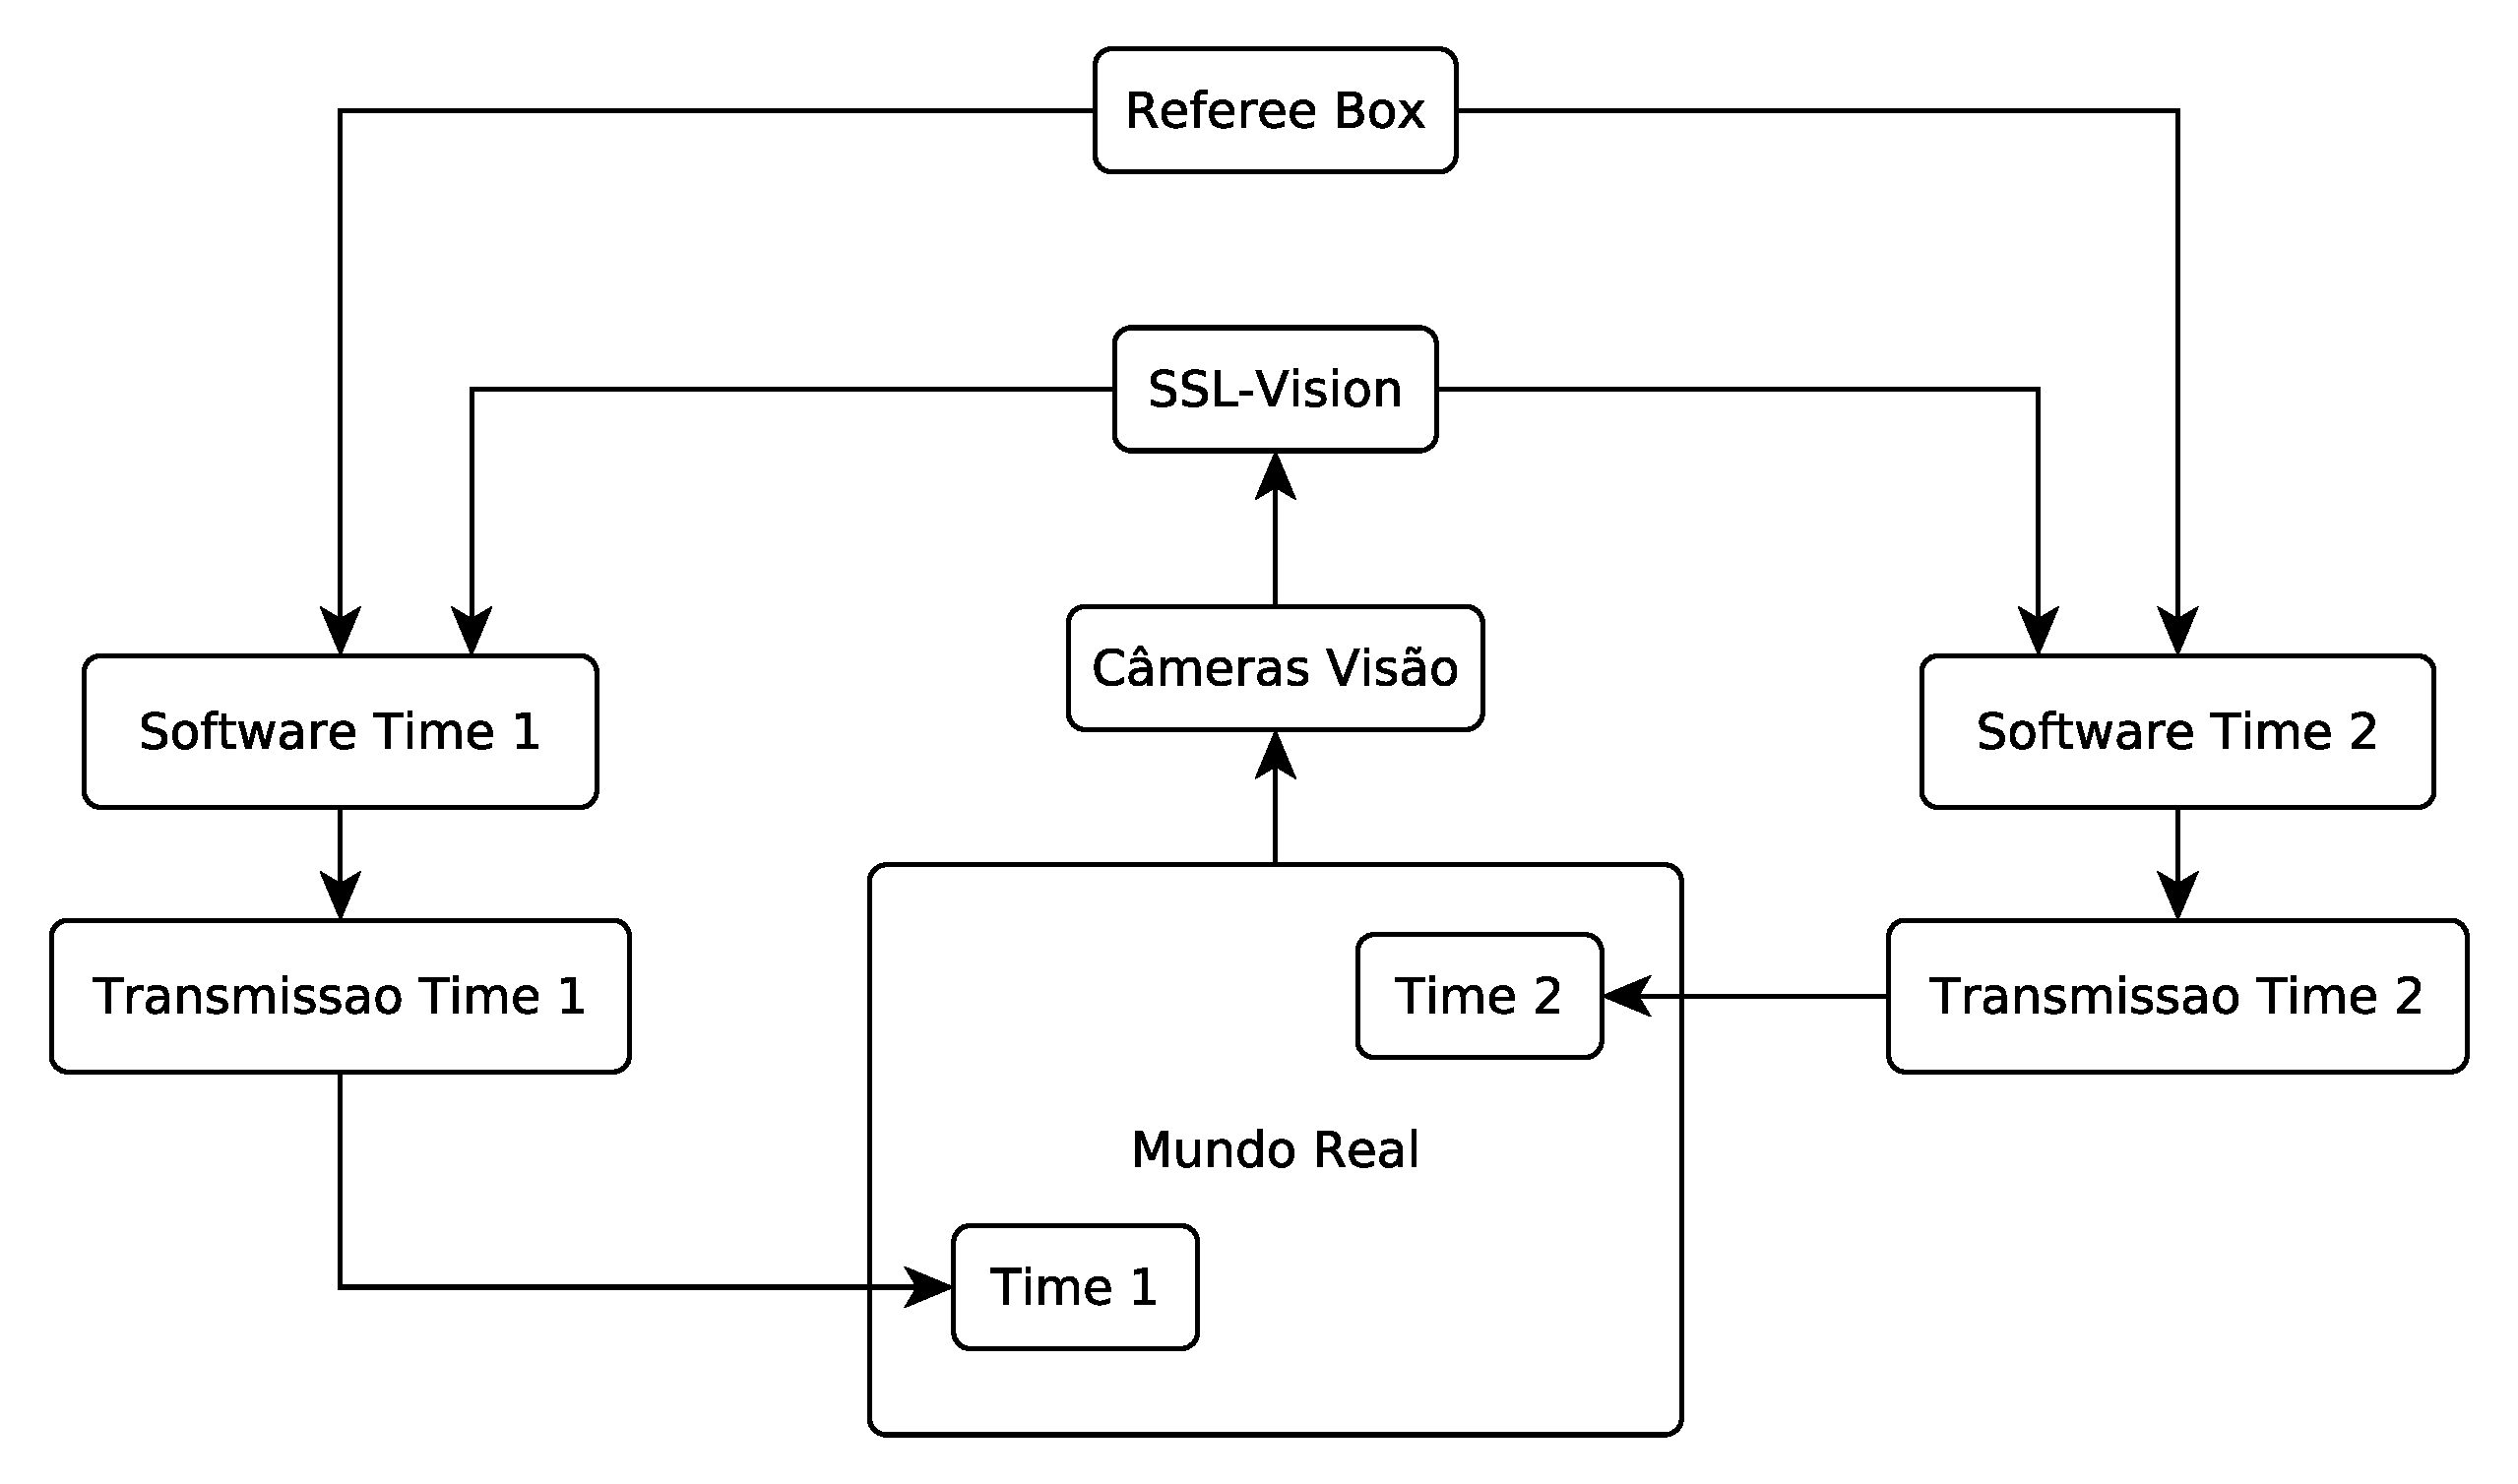
\includegraphics[width= 0.8\linewidth]{img/arq_ssl}
    \caption{Arquitetura básica da SSL}
  \end{figure}
}

\frame{%
  \frametitle{SSL}
  \begin{figure}[thpb]
    \centering
    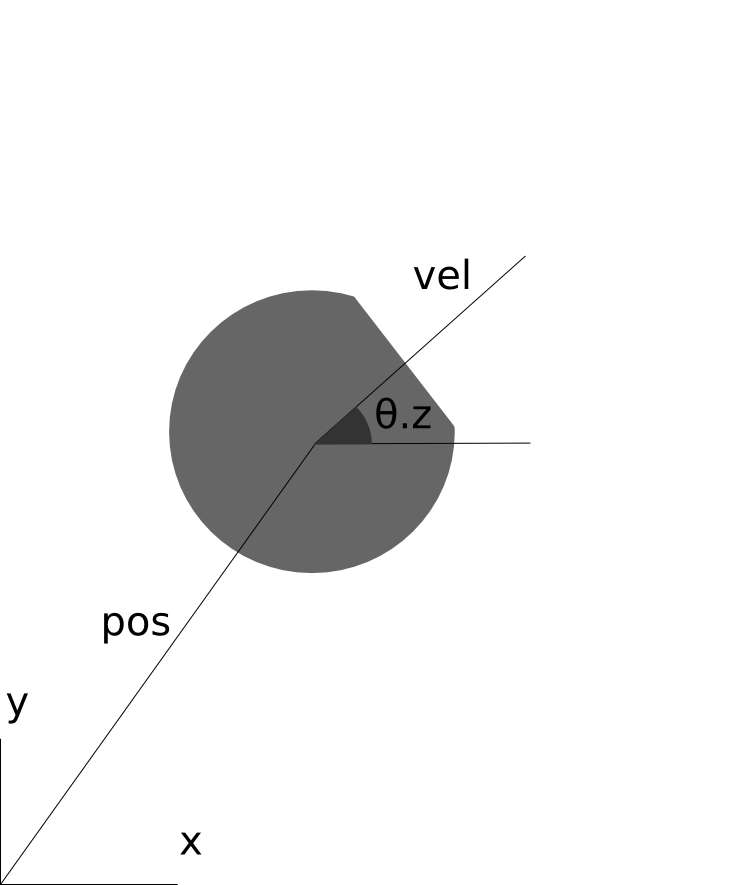
\includegraphics[width=0.3\linewidth]{img/rob_data}
    \caption{Parâmetros de estádo mutáveis do robô}
  \end{figure}
}

\subsection{Discretização}
\frame{%
  \frametitle{Discretização}
  \begin{block}{}
    \begin{itemize}
      \item Representação do jogo
      \begin{itemize}
        \item Posse de bola
        \item Ações Consideradas
      \end{itemize}

      \item Execução do planejamento: pyroboime
    \end{itemize}
  \end{block}
}

\frame{%
  \frametitle{Ações Consideradas}
  \begin{block}{}
    \begin{itemize}
      \item Time no ataque (i.e., com a bola)
      \begin{itemize}
        \item $Mover(r)$
        \item $Chutar(r_{com{\ }bola})$
        \item $Passar(r,r_{com{\ }bola})$
      \end{itemize}

      \item Time na defesa (i.e., sem a bola)
      \begin{itemize}
        \item $Mover(r)$
      \end{itemize}
    \end{itemize}
  \end{block}
}

\subsection{Função Objetivo}
\frame{%
  \frametitle{Função Objetivo}
  \begin{block}{}
    \begin{itemize}
      \item $f_U = \sum c_i$
      \item $c_i$: custos e penalizações
      \begin{itemize}
        \item Custo da Abertura do Gol
        \item Distância Total das Ações $Mover(r)$
        \item Distância Máxima das Ações $Mover(r)$
        \item etc
      \end{itemize}
    \end{itemize}
  \end{block}
}

\subsection{Estratégia de Busca}
\frame{%
  \frametitle{Estratégia de Busca}
  \begin{figure}[H]
    \centering
    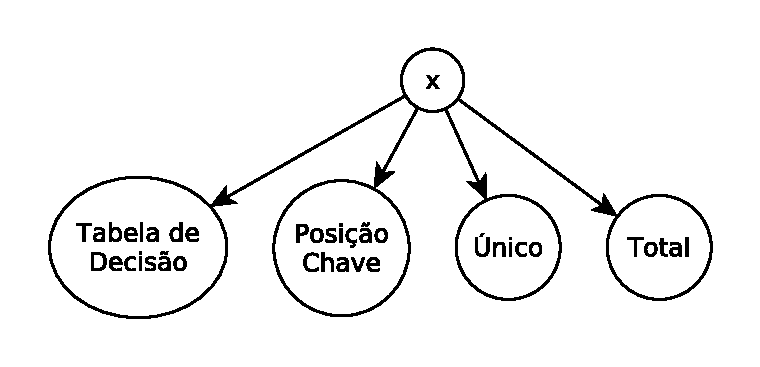
\includegraphics[width= 0.8\linewidth]{tab_dec}
    \caption{Ilustração da distribuição dos tabuleiros
             considerados no planejamento}\label{fig:estr_busca}
  \end{figure}
}

\frame{%
  \frametitle{Distribuição da Ação $Mover(r)$}
  \begin{figure}[H]
    \centering
    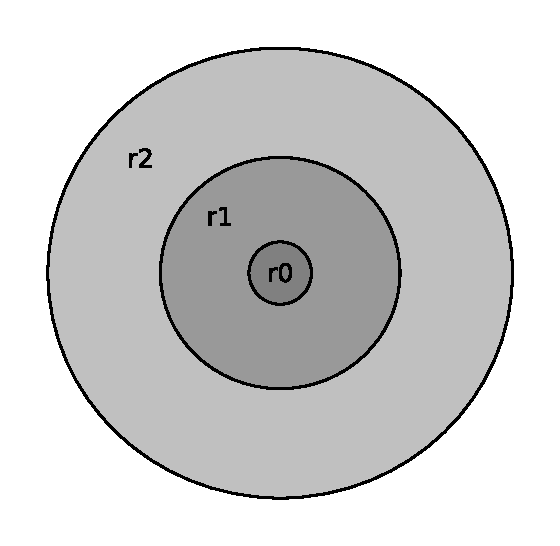
\includegraphics[width=0.5\linewidth] {distr_mov}
    \caption{Distribuição da Ação $Mover(r)$}\label{fig:distr_mov}
  \end{figure}
}

\frame{%
  \frametitle{Posição Chave}
  \begin{figure}[H]
    \centering
    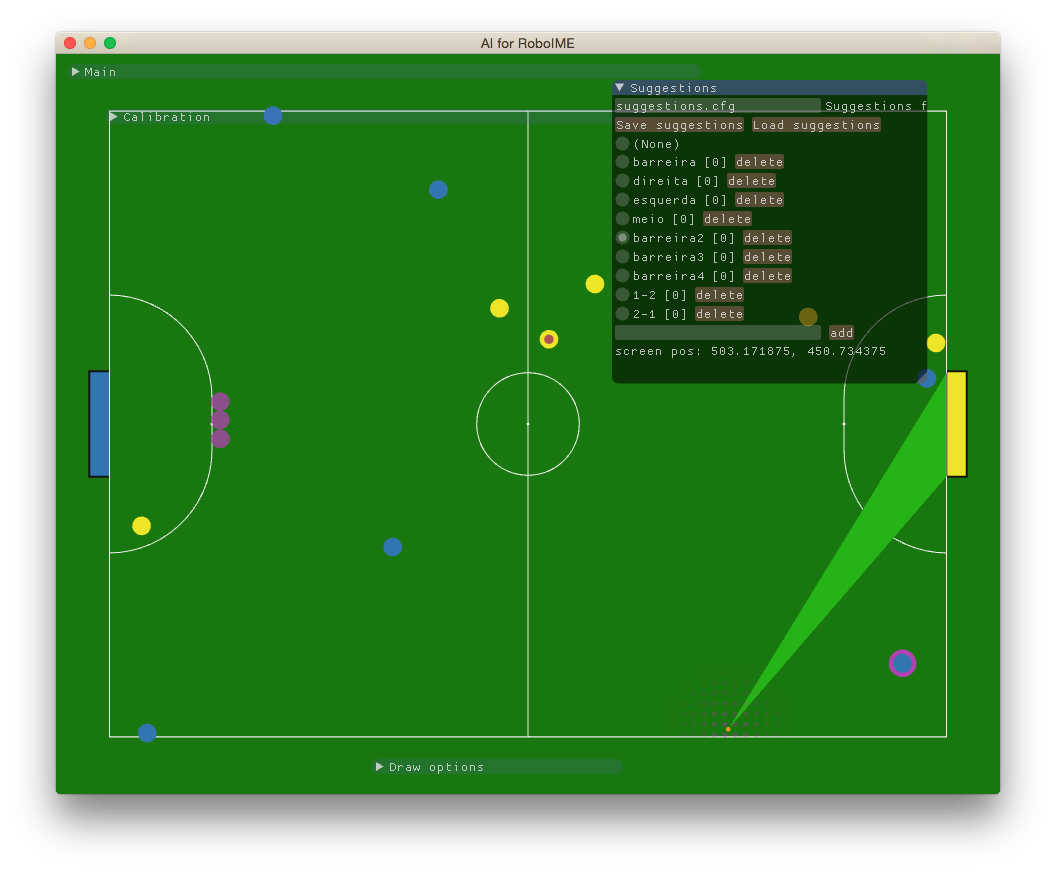
\includegraphics[width= 0.5\linewidth]{pos_chave_barreira}
    \caption{Sugestão de uma barreira (em rosa)}\label{fig:pos_chave_barreira}
  \end{figure}
}

\section{Arquitetura}
% - compet. ???
% - zmq / rede
% - evidenciar vantagens
% - python / c++
\frame{%
  \frametitle{Arquitetura}
  \begin{figure}
    \centering
    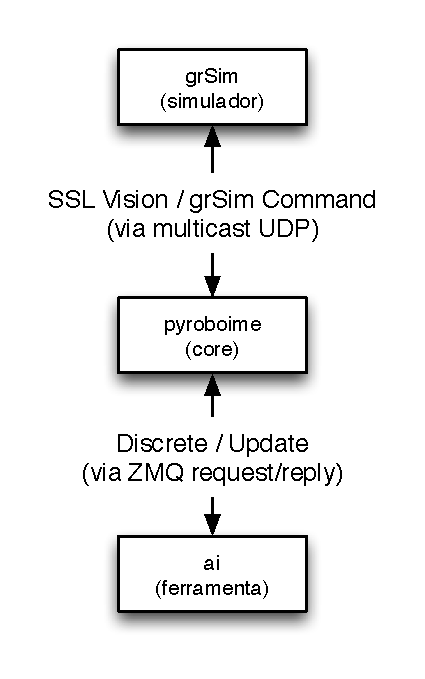
\includegraphics[width= 0.27\linewidth]{communication}
    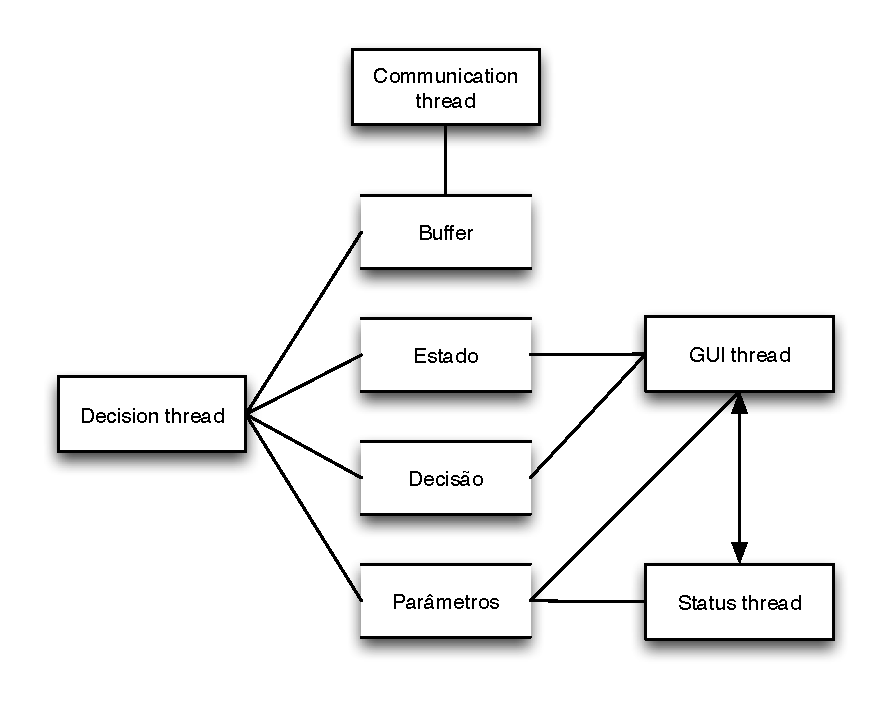
\includegraphics[width= 0.60\linewidth]{threads}
    \caption{Diagrama de comunicação entre os componentes
             (E) e de relação entre \textit{threads} e
             dados (D).}\label{fig:arch_threads}
  \end{figure}
}

\section{Resultados}
% Resultados
% - exemplo representacao
% - funcao de avaliacao e dados auxiliares
% - exemplo passe
% - execucao no grsim
\frame{%
  \frametitle{Resultados}
  \centering
  VIDEO
}

\section{Considerações finais}
\frame{%
  \frametitle{Considerações finais}
  \begin{figure}[H]
    \centering
    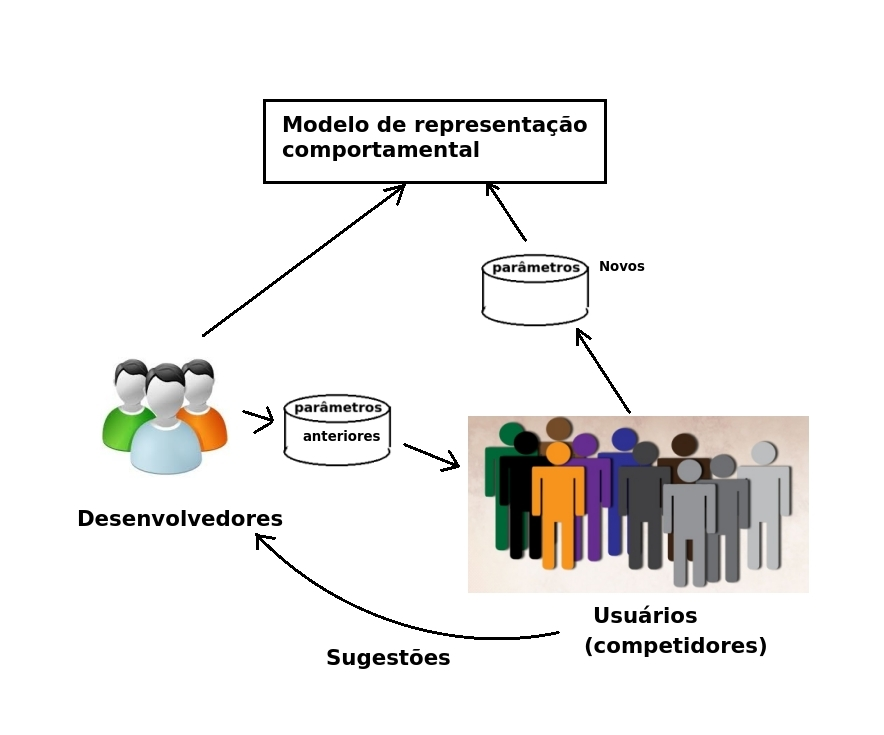
\includegraphics[width=0.6\linewidth]{mod_comp}
    \caption{Modelo de Competição para melhorar
             o time}\label{fig:mod_comp}
  \end{figure}
}

\section{Conclusão}
\frame{%
  \frametitle{Conclusão}
  \begin{block}{}
    \centering
    \begin{itemize}
      \item Foi desenvolvido um modelo abstrato do futebol de robôs, que
            foi base para o programa apresentado;
      \item A ferramenta criada atingiu os objetivos desejados, modificando o
            comportamento do time através da modificação dos parâmetros da
            função objetivo;
      \item A interface gráfica permite modificar esses parâmetros em tempo
            de execução.
    \end{itemize}
  \end{block}
}

\end{document}

% vim: tw=80 et ts=2 sw=2 sts=2 ft=tex
